
\subsubsection{Suposiciones}
A la hora de modelar el problema usando las herramientas vistas en la materia (diagrama de entidad--relación y diagrama de interacción de documentos)
realizamos unas pocas suposiciones sobre el problema, sobre todo en aspectos en los que la consigna era vaga. A continuación se encuentran las más importantes.

\begin{itemize}
\item Los estudiantes no pueden cambiarse de escuela a lo largo de su carrera (por lo tanto tampoco de país).
\item Los árbitros no pueden cambiarse de país a lo largo de su carrera.
\item Los enfrentamientos no pueden empatarse.
\end{itemize}

\subsubsection{Modelos relacionales}
Los diagramas son muy similares a los del Trabajo Práctico 1, y se encuentran en las páginas siguientes.

Agregamos una entidad Enfrentamiento, que modela los enfrentamientos para aquellas disciplinas que los tienen (por ejemplo Combate). Aquellas disciplinas que no tengan enfrentamientos (por ejemplo, Salto) no tendrán enfrentamientos.

Además, convertimos a la entidad Categoría (que contiene toda la información de la categoría de una competencia: edad permitida, dan, género, etcétera) en una entidad débil, dado que no tiene sentido su existencia separada de una competencia.

\newpage

\begin{figure}[H]
 \centering
 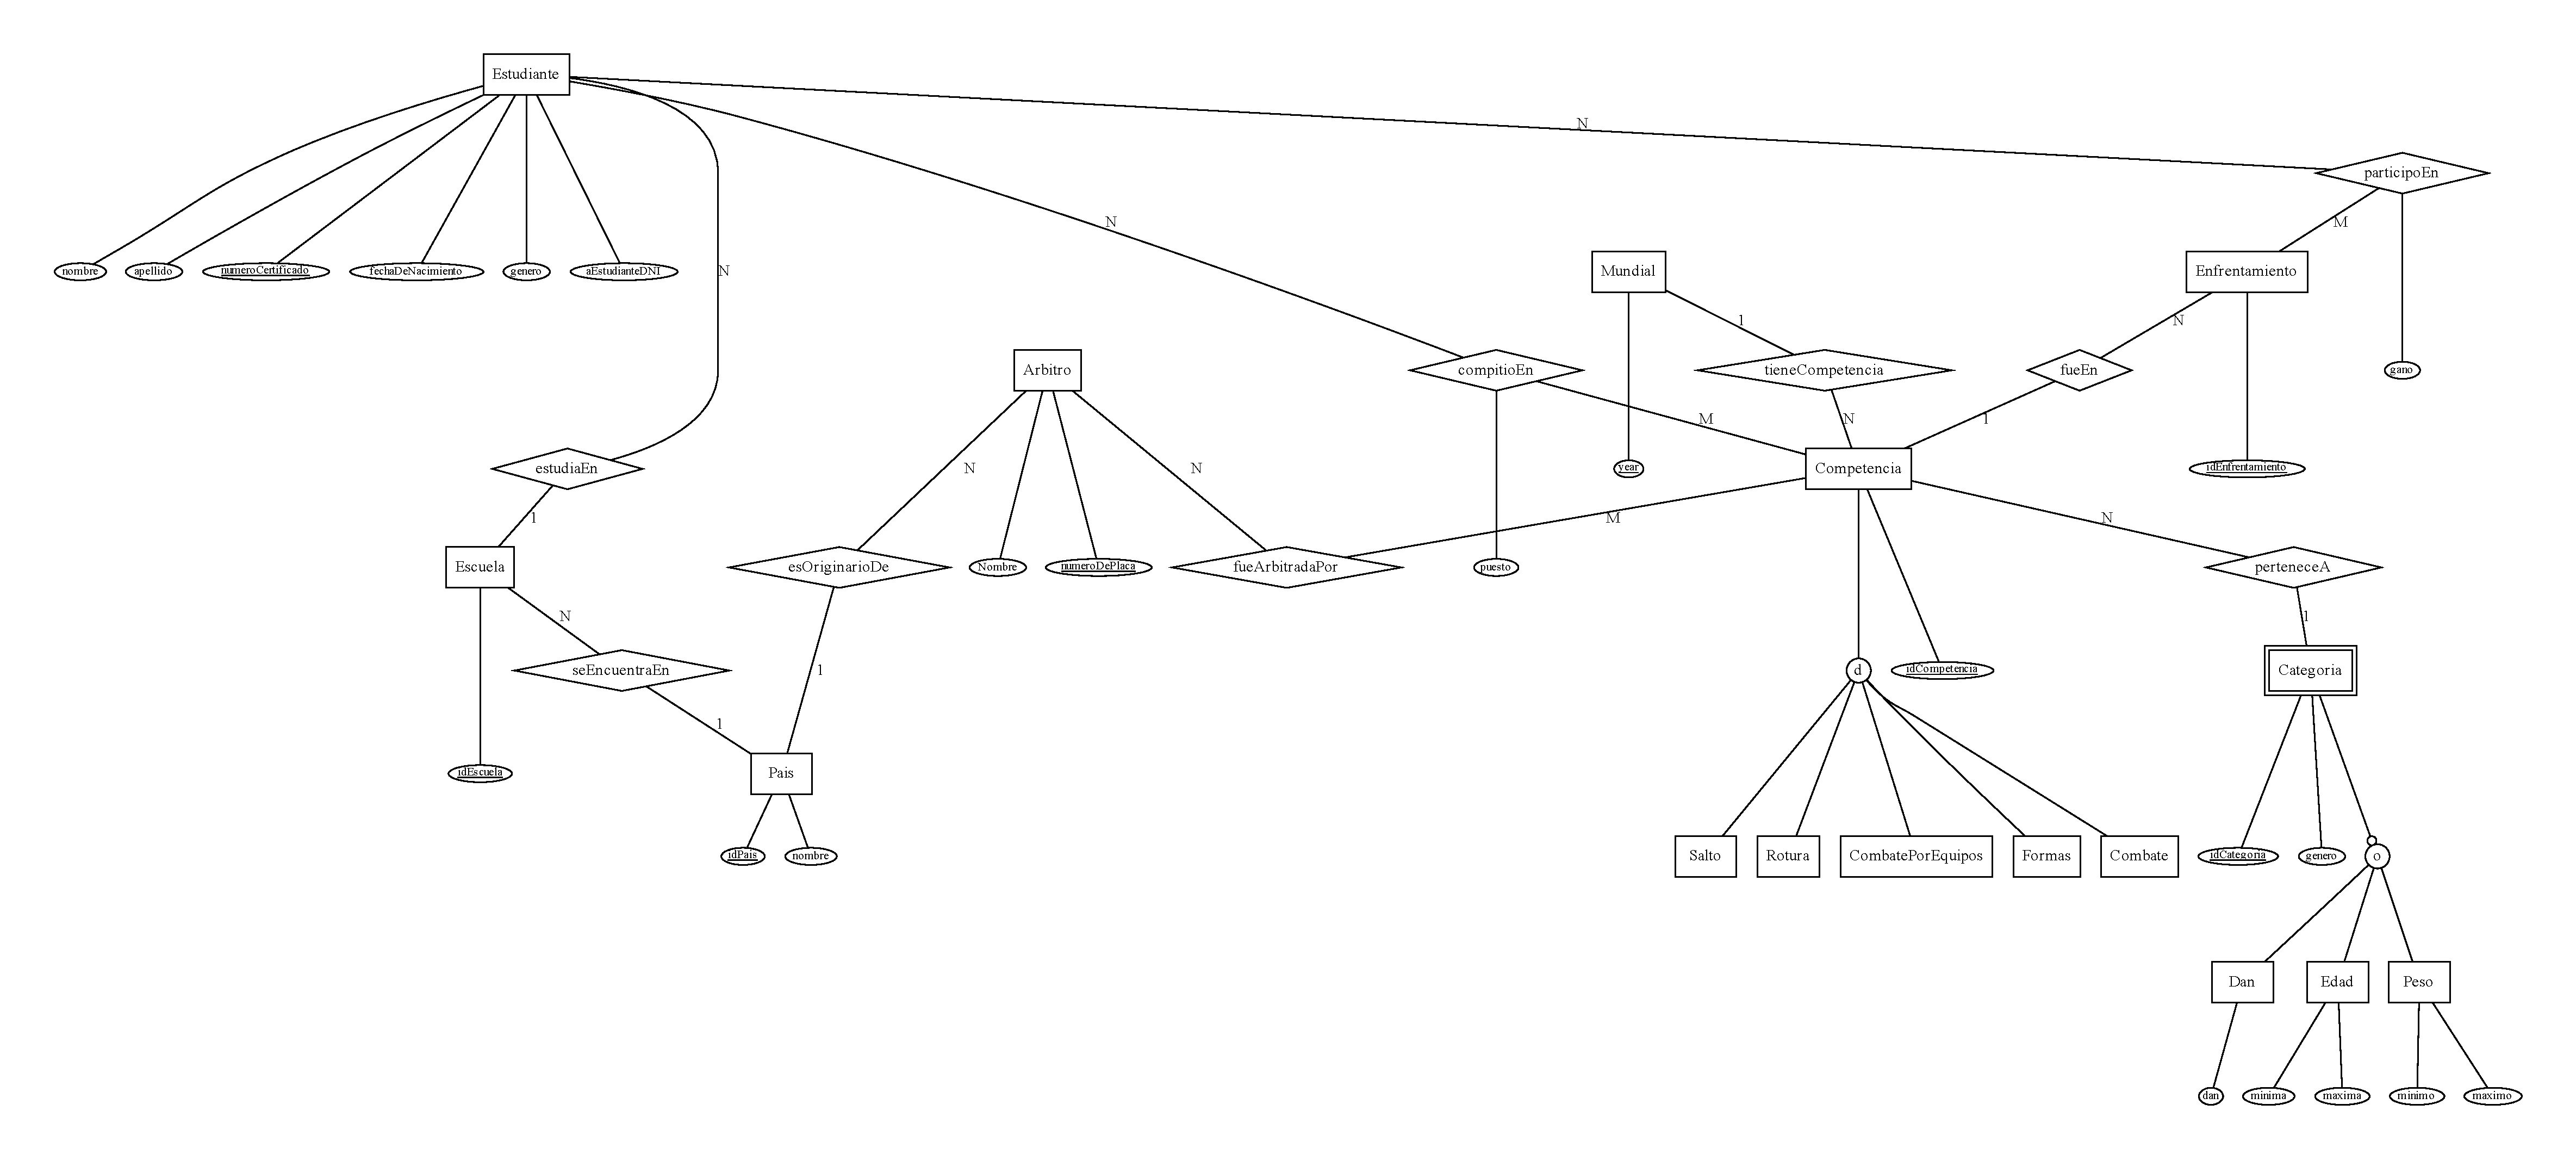
\includegraphics[angle=90,height=23cm]{../mer/mer-dot.pdf}
 \caption{Diagrama de Entidad--Relacion. Se puede hacer zoom en el pdf para ver mejor.}
\end{figure}

\begin{figure}[H]
  \centering
  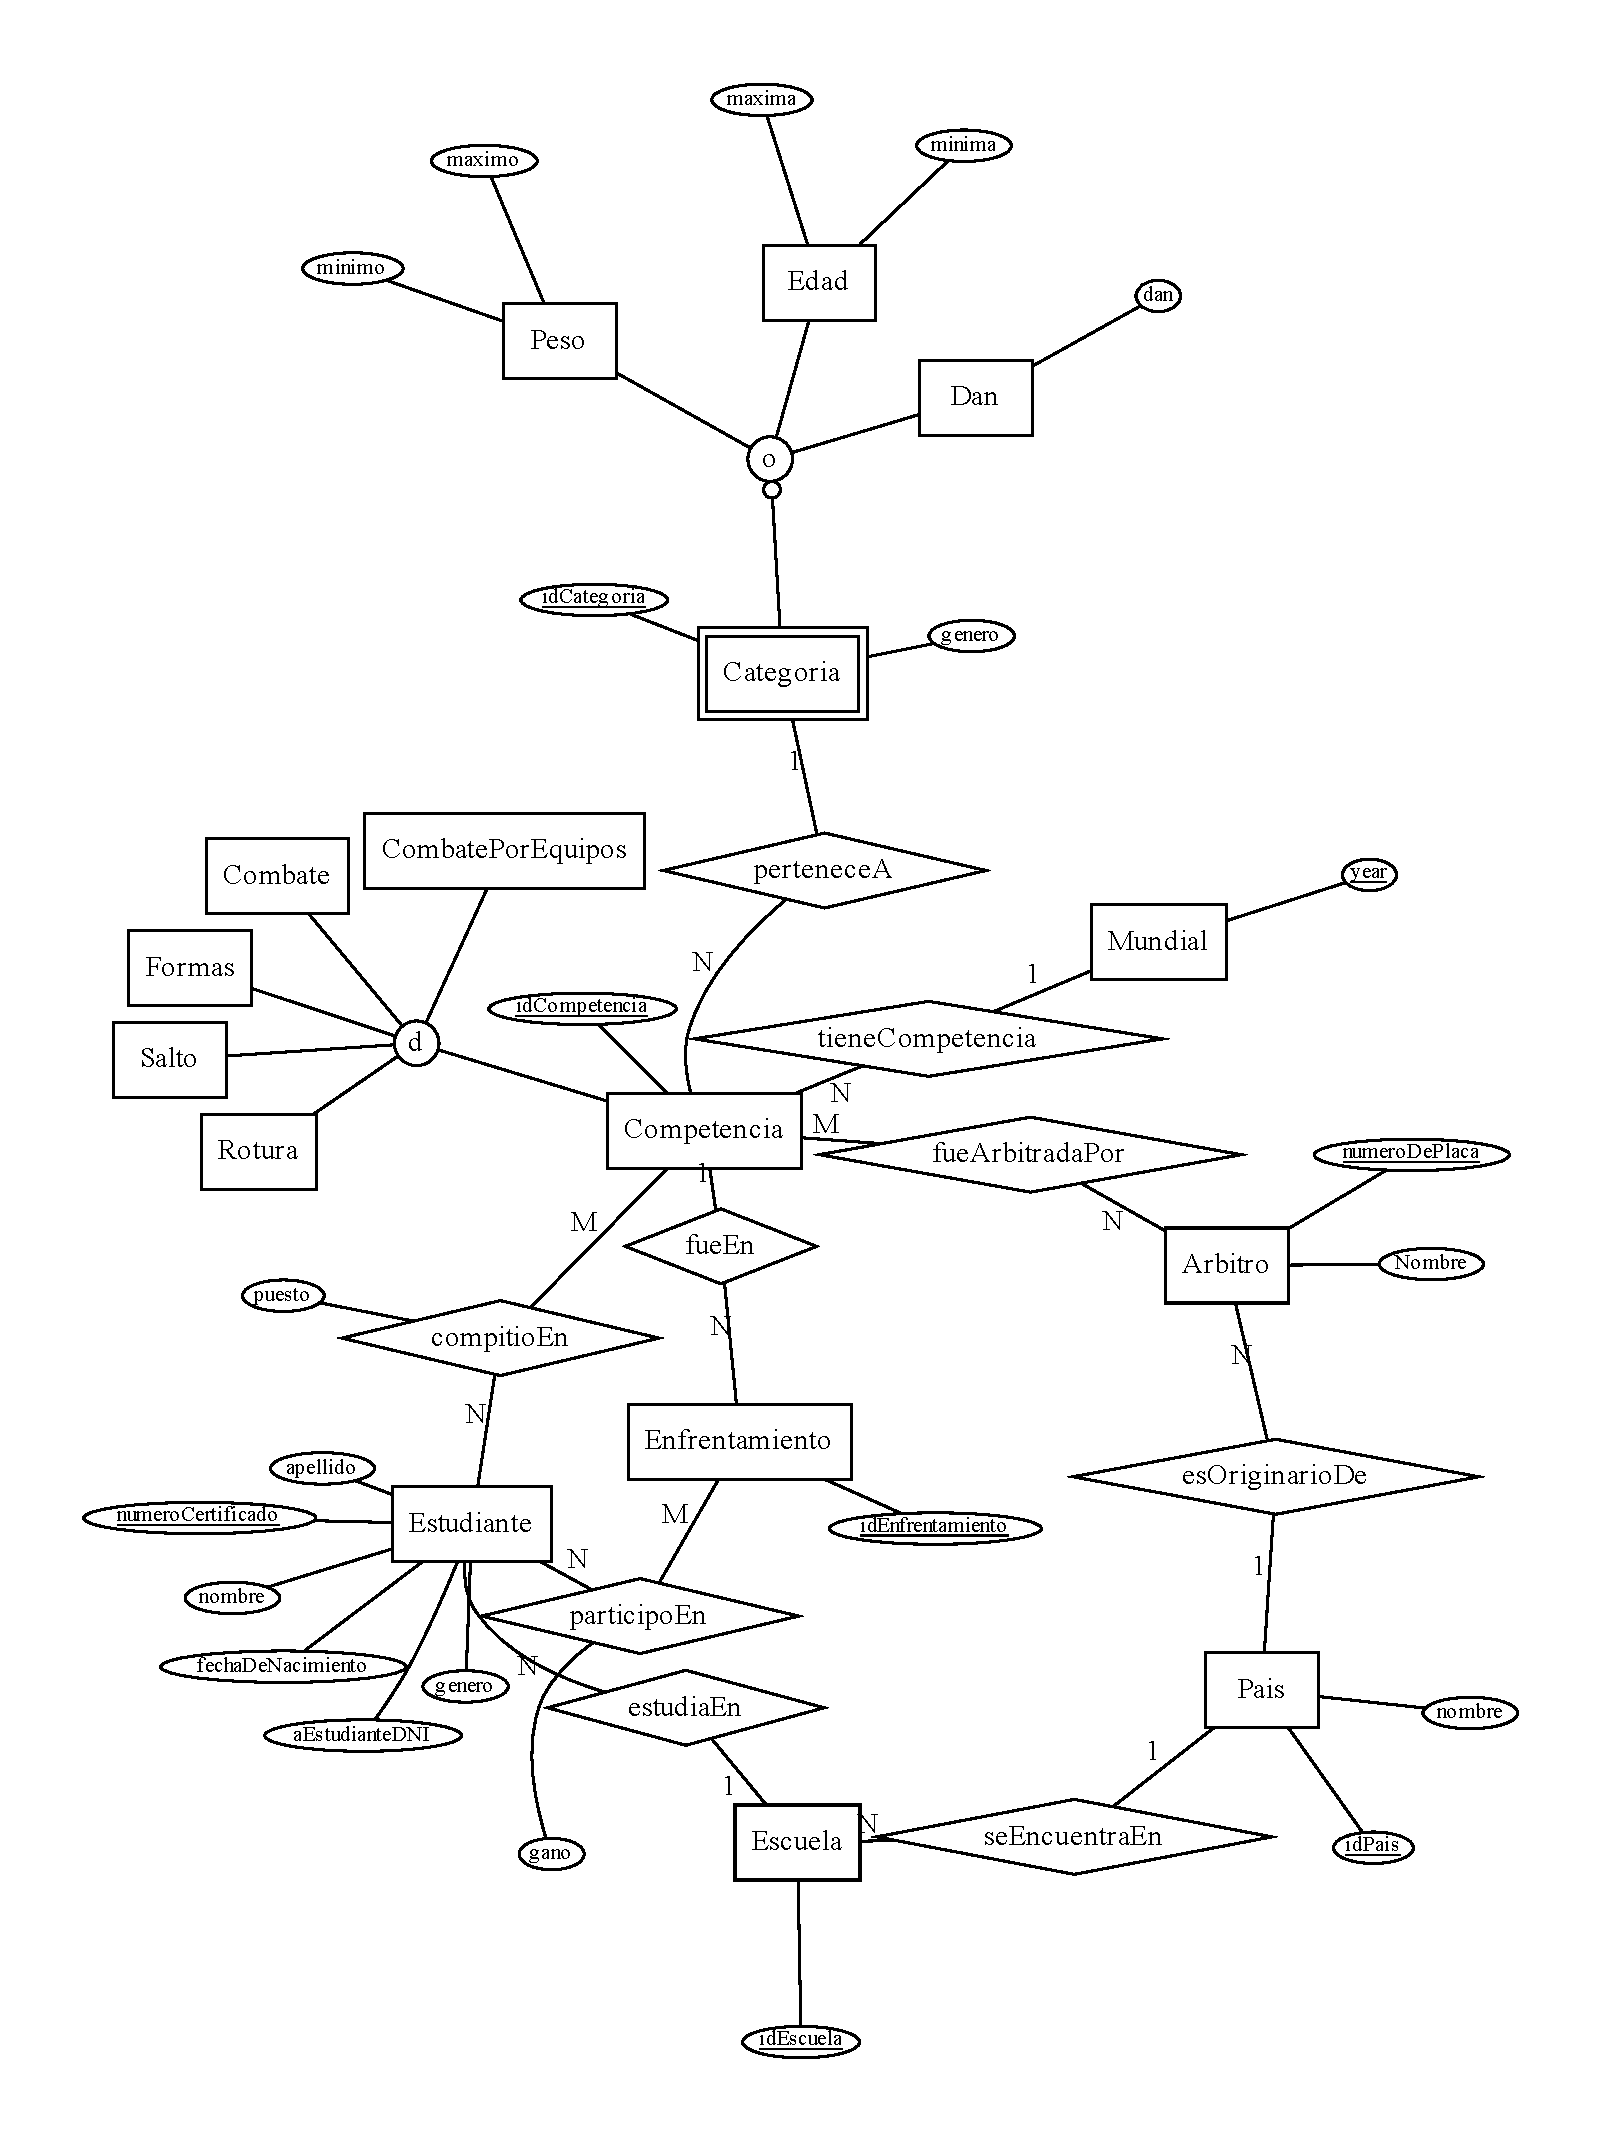
\includegraphics[width=\textwidth]{../mer/mer-neato.pdf}
  \caption{Diagrama de Entidad--Relación. Es el mismo diagrama que antes pero con otra disposición espacial.}
\end{figure}


